\section{Projekt aplikacji}
\subsection{Założenia}
Założenia aplikacji:
\begin{itemize}
    \item możliwość utworzenia konta i~zalogowania się na nie,
	\item możliwość dodawania zdjęć z opisem (tagami),
    \item możliwość wyszukiwania zdjęć po formacie,
    \item możliwość wyszukiwania zdjęć po rozmiarze,
    \item możliwość wyszukiwania zdjęć po kategorii,
    \item możliwość wyszukiwania zdjęć po tagach.
\end{itemize}

\subsection{Architektura}
Ze względu na specyfikę aplikacji wybrano architekturę klient-serwer. Część serwerowa umożliwia przechowywanie informacji o~zdjęciach i~użytkownikach, zaś część kliencka pozwala na przeglądanie zdjęć oraz wyszukiwanie ich według określonych kryteriów. Informacje o~użytkownikach i~zdjęciach będą zapisywane w~bazie danych MySQL, znajdującej się na tej samej maszynie co część serwerowa. 

Klient do działania będzie wymagał dostępu do Internetu oraz przeglądarki internetowej. Aplikacja pobierze zdjęcia z~bazy danych za pośrednictwem serwera. Obrazy nie będą fizycznie przechowywane w~bazie danych - w tabeli zostanie zapisany jedynie odnośnik do lokalizacji na serwerze.

Połączenie pomiędzy klientem a serwerem zostało oparte
na architekturze REST.
Serwer zaprojektowano i~podzielono na warstwy tak, aby dostęp do niego był możliwy niezależnie od rodzaju klienta. Wydzielono warstwę danych, logiki, a także warstwę udostępniającą interfejs REST, który serwuje dane w~formacie JSON. W realizowanym projekcie komunikacja pomiędzy klientem, a serwerem będzie odbywała się poprzez ten interfejs, za pomocą żądań HTTP. Ogólny schemat przetwarzania takiego żądania przedstawiono na rysunku \ref{fig:requestProcessing}. 
\begin{figure}[ht]
	\centering
	\includegraphics[width = 12cm]{images/requestProcessing.png}
	\caption{Przetwarzanie zapytania na serwerze
		\newline Źródło: opracowanie własne}
	\label{fig:requestProcessing}
\end{figure}
\subsection{Interfejs REST}
Tworząc interfejs oparty na architekturze REST należało
wyodrębnić zasoby, które będą udostępniane klientom. Wyróżniono trzy: użytkownicy, zdjęcia, tagi. Każdemu z~zasobów
został przypisany adres:
\begin{itemize}
        \item \texttt{http://adres.serwera/TestProject/api/user/} udostępnia zasób ,,użytkownicy'' (tabela \ref{table:restUsers}),
        \item \texttt{http://adres.serwera/TestProject/api/image/} udostępnia zasób ,,zdjęcia'' (tabela \ref{table:restImages}),
        \item \texttt{http://adres.serwera/TestProject/api/tag/} udostępnia zasób ,,tagi'' (tabela \ref{table:restTags}).
\end{itemize}

\begin{table}[ht]
	\centering
	\caption{Adresy zasobu ,,użytkownicy''}
	\label{table:restUsers}
 \begin{tabular}{|l|c|c|}
	\hline 
	adres & metoda & operacja  \\
	\hline 
	\texttt{/user/} & POST &  rejestracja użytkownika  \\
	\hline 	
	\texttt{/user/login}  & POST & logowanie użytkownika  \\	
	\hline 
    \texttt{/user/login}  & DELETE & wylogowanie użytkownika \\
	\hline 
\end{tabular}
\end{table}

\begin{table}[ht]
	\centering
	\caption{Adresy zasobu ,,zdjęcia''}
	\label{table:restImages}
 \begin{tabular}{|l|c|c|}
	\hline 
	adres & metoda & operacja  \\
	\hline 
	\texttt{/image/} & GET &  pobranie wszystkich zdjęć \\
	\hline 
    \texttt{/image/} & POST &  wgranie zdjęcia \\
    \hline 
	\texttt{/image/\{id\}} & GET & pobranie informacji o~zdjęciu o~id=\{id\} \\	
	\hline 
	\texttt{/image/details/\{id\}} & GET & pobranie dokładnych informacji o~zdjęciu o~id=\{id\} \\	
	\hline 
	\texttt{/image/size/{size}} & GET & wyszukiwanie zdjęć po rozmiarze=\{size\}\\
	\hline 
	\texttt{/image/user/{userID}} & GET & wyszukiwanie zdjęć użytkownika o~id=\{userID\} \\
    \hline 
    \texttt{/image/extension/{extension}} & GET & wyszukiwanie zdjęć po rozszerzeniu=\{extension\} \\
    \hline 
    \texttt{/image/tag/{tag}} & GET & wyszukiwanie zdjęć z tagiem=\{tag\}\\
    \hline 
    \texttt{/image/category/{category}} & GET & wyszukiwanie zdjęć z kategorii=\{category\}\\
    \hline 
\end{tabular}
\end{table}

\begin{table}[!ht]
\centering
\caption{Adresy zasobu ,,tagi''}
\label{table:restTags}
\begin{tabular}{|l|c|c|}
	\hline 
	adres & metoda & operacja  \\
	\hline
	\texttt{/tag/All} & GET & pobranie wszystkich tagów \\
	\hline
\end{tabular}
\end{table}

\section{Baza danych}
W celu przechowywania danych zaprojektowano bazę danych przedstawioną na rysunku \ref{fig:database}. Sama baza danych zostanie stworzona z~klas modelu dzięki użyciu standardu JPA. Na bazę składa się pięć tabel, ich szczegółowy opis przedstawiono poniżej.
\begin{itemize}
	\item Image - tabela przechowująca informacje o~zdjęciach
	\begin{itemize}
		\item id - identyfikator
		\item URL - adres URL do lokalizacji zdjęcia na serwerze
		\item extension - rozszerzenie
		\item size - rozmiar zdjęcia
		\item width - szerokość zdjęcia
        \item height - wysokość zdjęcia
        \item categoryName - klucz obcy do tabeli Category
        \item description - opis zdjęcia
        \item userId - klucz obcy do tabeli User
	\end{itemize}
	\item User - tabela przechowująca dane o~użytkownikach
	\begin{itemize}
		\item id - identyfikator
		\item username - login użytkownika
		\item password - hash hasła użytkownika
		\item token - token uwierzytelniający użytkownika
	\end{itemize}
	\item Category - tabela przechowująca informacje o~kategoriach
	\begin{itemize}
		\item name - nazwa kategorii
	\end{itemize}
    \item Tag - tabela przechowująca informacje o~tagach
    \begin{itemize}
        \item name - nazwa tagu
    \end{itemize}
	\item TagImage - tabela łącząca zdjęcie z~tagiem, przechowuje informacje o~tagach przypisanych do zdjęć
	\begin{itemize}
		\item id - identyfikator
		\item imageId - klucz obcy do tabeli Image
		\item tagName - klucz obcy do tabeli Tag
	\end{itemize}
\end{itemize}

\begin{figure}[ht]
	\centering
	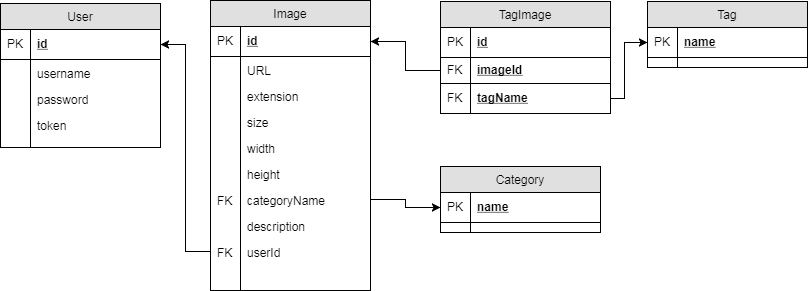
\includegraphics[width=12cm]{images/bazaDanych}
	\caption{Schemat bazy danych
		\newline Źródło: opracowanie własne}
	\label{fig:database}
\end{figure}
